% Three-page progress report: AMOC adjoint sensitivity in the 2° OMIP ocean (NumericalEarth, Reactant + Enzyme).
% Build with `latexmk -pdf omip_amoc_adjoint_report.tex` in this directory. Detail: omip_amoc_adjoint.tex.
\documentclass[10pt]{article}

\usepackage[margin=0.85in]{geometry}
\usepackage{amsmath, amssymb}
\usepackage{booktabs}
\usepackage{graphicx}
\usepackage{hyperref}
\usepackage{siunitx}
\usepackage{enumitem}
\usepackage{caption}
\usepackage{titlesec}
\titlespacing*{\section}{0pt}{7pt}{2pt}
\setlist{nosep, leftmargin=1.2em}
\captionsetup{font=small, skip=4pt}
\setlength{\parskip}{3pt}
\setlength{\parindent}{0pt}

\newcommand{\gvec}{\mathbf{g}}
\newcommand{\uu}{\mathbf{u}}

\title{\vspace{-2.2em}\textbf{Adjoint sensitivity of the AMOC at \ang{26.5}N to surface forcing in a
       differentiable 2\textdegree{} OMIP ocean}\vspace{-0.6em}}
\date{Progress report, \today\vspace{-1.2em}}

\begin{document}
\maketitle

\section*{Summary}

I compute the gradient of the Atlantic overturning at \ang{26.5}N with respect to the surface forcing
of a global 2\textdegree{} ocean. The gradient is the Enzyme reverse-mode adjoint of the
Reactant-compiled \textsc{Oceananigans} model, set up through NumericalEarth's OMIP configuration.
\begin{itemize}
  \item \textbf{Windows up to 30 days work, at a cost that does not grow with length.} One time step and
        its reverse pass are compiled once and run on a binomial (Revolve) checkpoint schedule. The compile
        takes about \SI{28}{min} at any window length. A compiled 30-day gradient
        ($\sim\!10^8$ controls) then costs \SI{104}{s} on one A100.
  \item \textbf{The adjoint is exact.} Finite differences agree with it to \numrange{e-9}{e-8} (relative) at
        8, 84 and 360 steps, inside the region where the objective is smooth.
  \item \textbf{Past about a day, the objective is only piecewise smooth.} Discrete switches in the forward
        model (most likely CATKE's mixing branches) make $J$ jump by \SIrange{e-7}{e-3}{Sv}. Small-step Taylor
        tests therefore fail, but at finite amplitude (\SIrange{0.25}{1}{m/s}) the gradient predicts the
        30-day response to within \SIrange{0.05}{2}{\percent}.
  \item \textbf{Freezing the mixing in the adjoint is not needed at 30 days.} The frozen gradient is close
        in direction (cosine 0.994), slightly less accurate and no cheaper. It does change the large-scale
        sums, for example the response to a uniform meridional wind.
  \item \textbf{Next: Pillar et al.\ (2016)-style lead-time maps.} 90-day and 1-year windows forced by ECCO4
        fluxes are running.
\end{itemize}

\section*{Configuration}

\begin{center}\small
\begin{tabular}{@{}lp{0.74\textwidth}@{}}
\toprule
Grid & \textsc{TripolarGrid} $180\times60\times20$ ($\approx\ang{2}$), exponential spacing to \SI{5500}{m};
       ETOPO bathymetry, immersed boundary \\
Dynamics & hydrostatic Boussinesq, TEOS-10; split Runge--Kutta 3, $\Delta t = \SI{2}{h}$; split-explicit free surface \\
Numerics & WENO momentum (5th order) and tracer (7th order) advection \\
Closures & CATKE vertical mixing; GM/Redi ($\kappa = \SI{800}{m^2/s}$); biharmonic viscosity \\
Forcing (A) & JRA55 repeat-year 3-hourly atmosphere, OMIP-2 bulk formulae; control = \SI{10}{m} winds $(u_{10}, v_{10})$
              on every slice; WOA initial state, at rest \\
Forcing (B) & ECCO4 monthly wind stress, net heat flux and net freshwater flux, from the 1993-01 ECCO4 state;
              control = all four fluxes on every monthly slice (Pillar's controls) \\
Objective & residual overturning $\psi$ at \SI{1000}{m} across a staircase section along \ang{26.5}N, \ang{80}W--\ang{14}W
            (RAPID line); at the window's end (A), or averaged over its last 30 days (B) \\
Backend & Float64, Reactant 0.2.303 / XLA, one NVIDIA A100 (TACC Lonestar6) \\
\bottomrule
\end{tabular}
\end{center}

\paragraph{Objective.} With signed, wet-masked face areas $W$ of the staircase and section area $a_k$ per level,
\begin{equation*}
T_k = \sum_{ij} \big(W^{v}_{ijk} v_{ijk} + W^{u}_{ijk} u_{ijk}\big), \quad
\tilde T_k = T_k - \frac{\sum_{k'} T_{k'}}{\sum_{k'} a_{k'}}\, a_k, \quad
J = -10^{-6} \sum_{k \le k_{\text{ref}}} \tilde T_k \;\;[\si{Sv}].
\end{equation*}
$J$ is linear in the velocities. On the tripolar grid a single grid row drifts from \ang{28}N to \ang{34}N
across the Atlantic, which is why the section follows a staircase of faces.

\paragraph{Adjoint.} Five functions are compiled once: the diagnostic refresh, one coupled step, and the
reverse passes of the refresh, the step and $J$. The host drives them on the Revolve schedule
(\texttt{Checkpointing.jl}), and each checkpoint is a host copy of the model's device memory. With this,
the compile cost no longer grows with the window: differentiating the whole window as one module took
\SI{48}{min} to compile at only 2 steps, and a rolled loop needed \SI{73}{GiB} of shadow state. The
averaged objective seeds the adjoint after each of the last $n_{\text{avg}}$ reverse steps, which needs no
extra state because $J$ is linear. An optional \emph{frozen-mixing} mode passes CATKE's diffusivities
through a stop-gradient: the forward model is unchanged, and the adjoint treats mixing as fixed, as
Pillar et al.\ do with KPP.

\section*{Verification}

\begin{center}\small
\begin{tabular}{@{}p{0.27\textwidth}rp{0.2\textwidth}p{0.38\textwidth}@{}}
\toprule
Window (forcing A unless noted) & $J$ [Sv] & Check & Result (relative error) \\
\midrule
1 step & $-14.35$ & Taylor; CPU twin & \num{6e-5}; primal vs.\ twin \num{7.5e-13} \\
2 steps (Revolve) & $-28.56$ & Taylor & \num{2e-7}; cosine to unrolled $\gvec$: $1 - \num{4e-10}$ \\
8 steps (16 h) & $-11.28$ & FD scan, 25 octaves & central \numrange{4e-9}{2e-8} \\
84 steps (1 week) & $-15.97$ & FD scan & central \num{4e-9}, $h \le \SI{2.4e-4}{m/s}$ \\
360 steps (30 days) & $+16.63$ & FD scan & forward \numrange{1e-6}{2e-5}, $h \le \SI{3e-5}{m/s}$ \\
8 steps, B, 4-step average & $-7.59$ & Taylor & \num{7.4e-4} (\num{5.5e-4} unaveraged) \\
\end{tabular}
\end{center}

\begin{figure}[h]
\centering
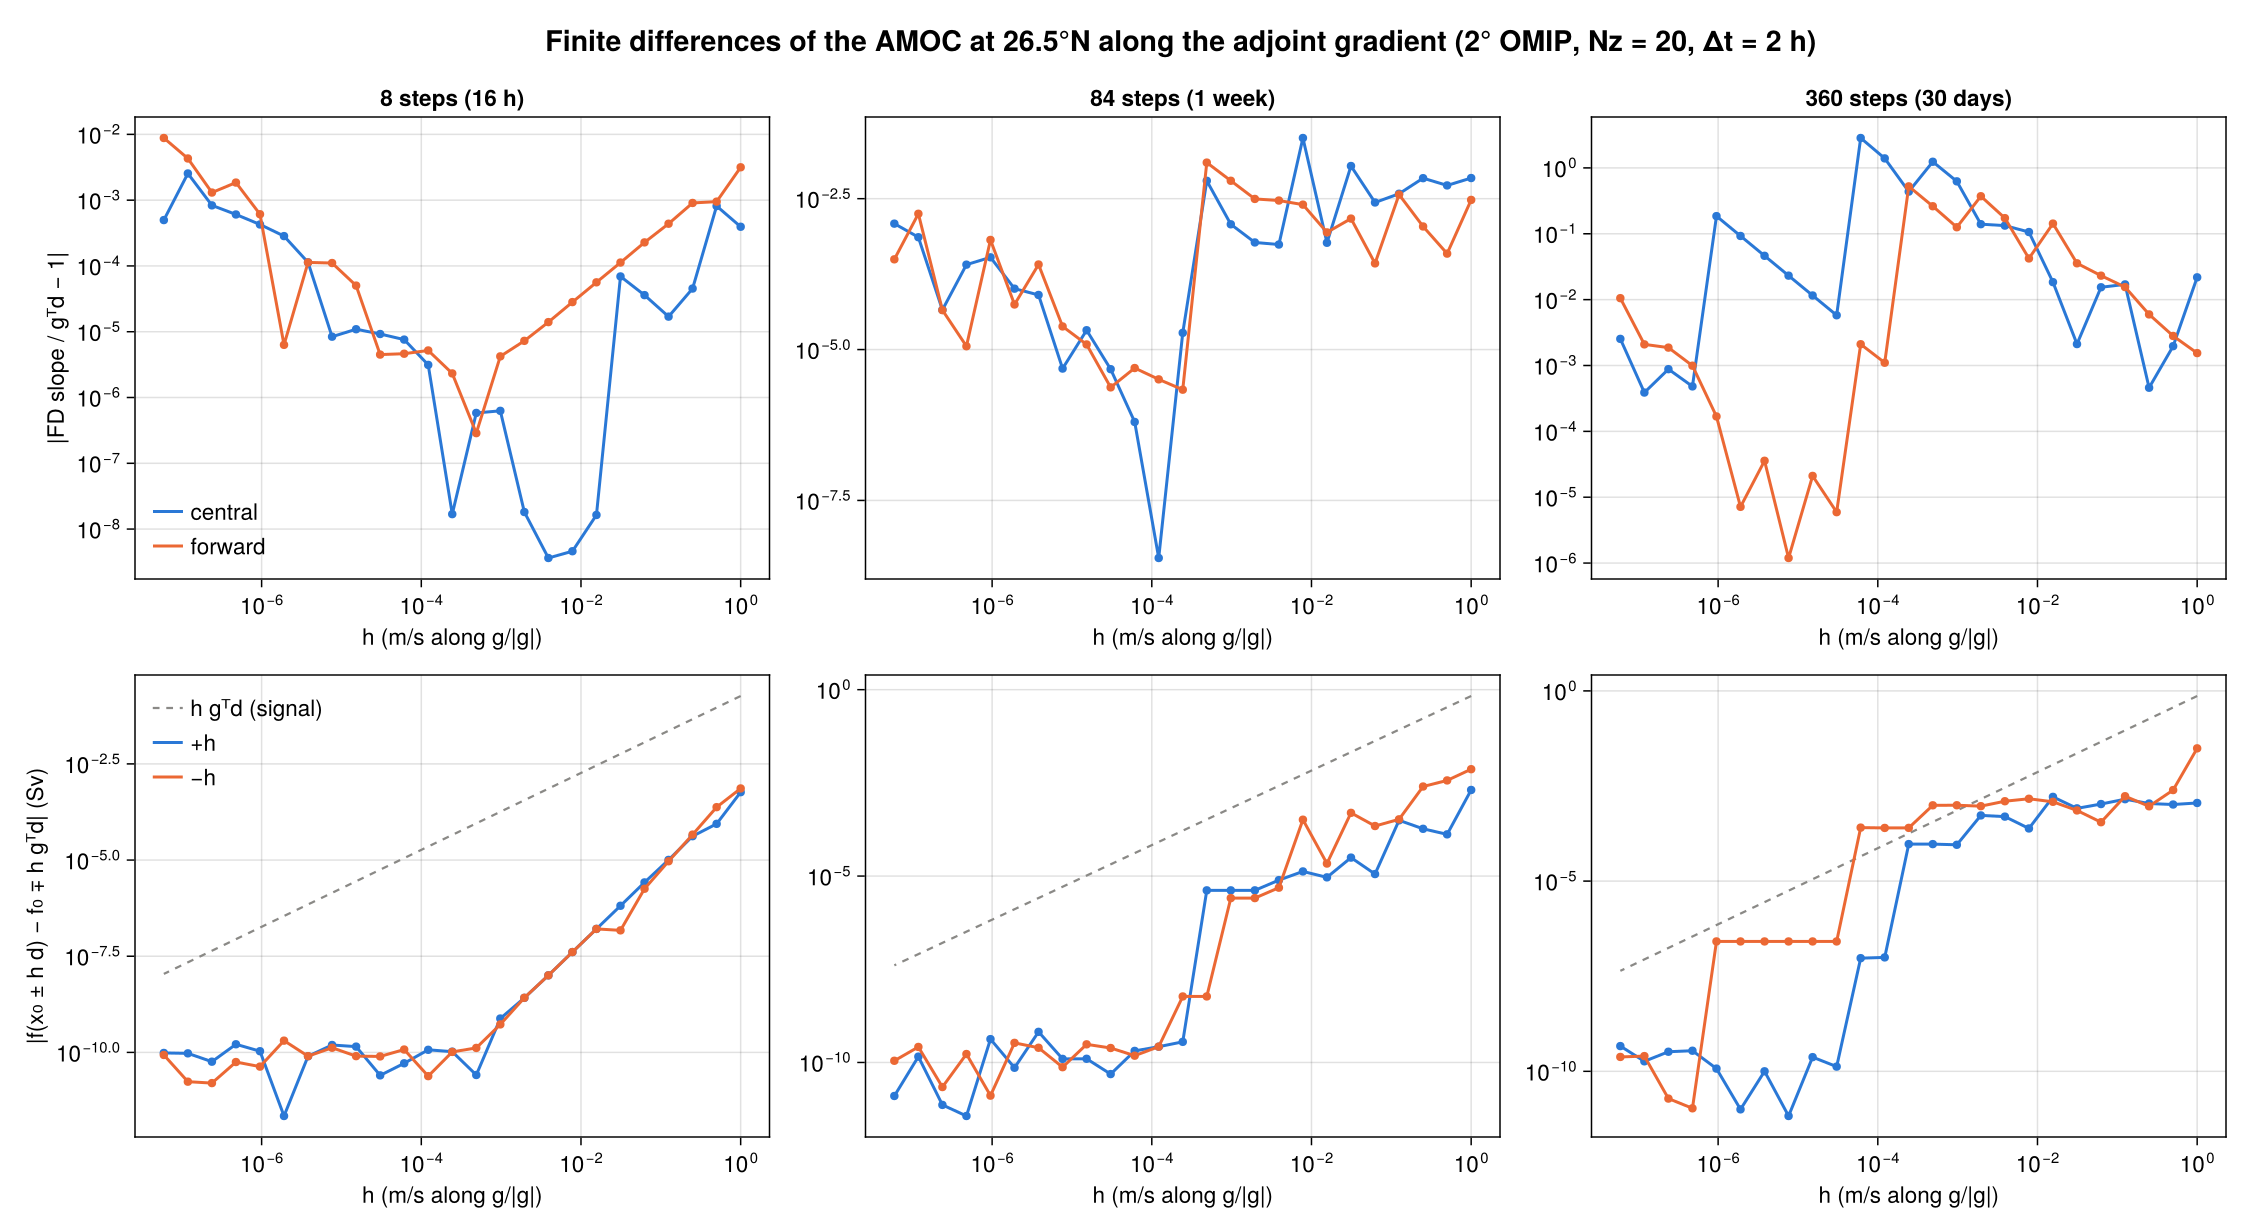
\includegraphics[width=0.86\textwidth]{figures/fd_scans_twodegree_nz20.png}
\caption{Finite differences of $J$ along $d = \gvec/\lVert\gvec\rVert$ at 8, 84 and 360 steps. Top: error of the
central and forward differences relative to $\gvec^{\mathsf T}d$. Bottom: residual of the linear prediction on
each side, with the signal $h\,\gvec^{\mathsf T}d$ dashed. A plateau as $h$ shrinks is a jump in $J$: none at 8
steps, \SIrange{e-6}{3e-4}{Sv} at 84, up to $\sim\!\SI{e-3}{Sv}$ at 360.}
\label{fig:fd}
\end{figure}

Below each jump the adjoint and finite differences agree to roundoff, and that smooth neighborhood
shrinks with the window ($h \lesssim \SI{2e-4}{m/s}$ at one week; on one side only \SI{5e-7}{m/s} at 30
days). The adjoint differentiates the branch the forward run took; this is the chaotic-adjoint behavior
of Lea et al.\ (2000). For sensitivity studies the relevant scale is finite amplitude. Over
$h = 0.25$--\SI{1}{m/s} the secant slope matches $\gvec^{\mathsf T}d$ to \num{4e-4} at 8 steps,
\numrange{5e-3}{7e-3} at 84, and \numrange{5e-4}{2e-2} at 360.

\section*{Results: 30-day sensitivity to the winds, full and frozen adjoint}

\begin{figure}[h]
\centering
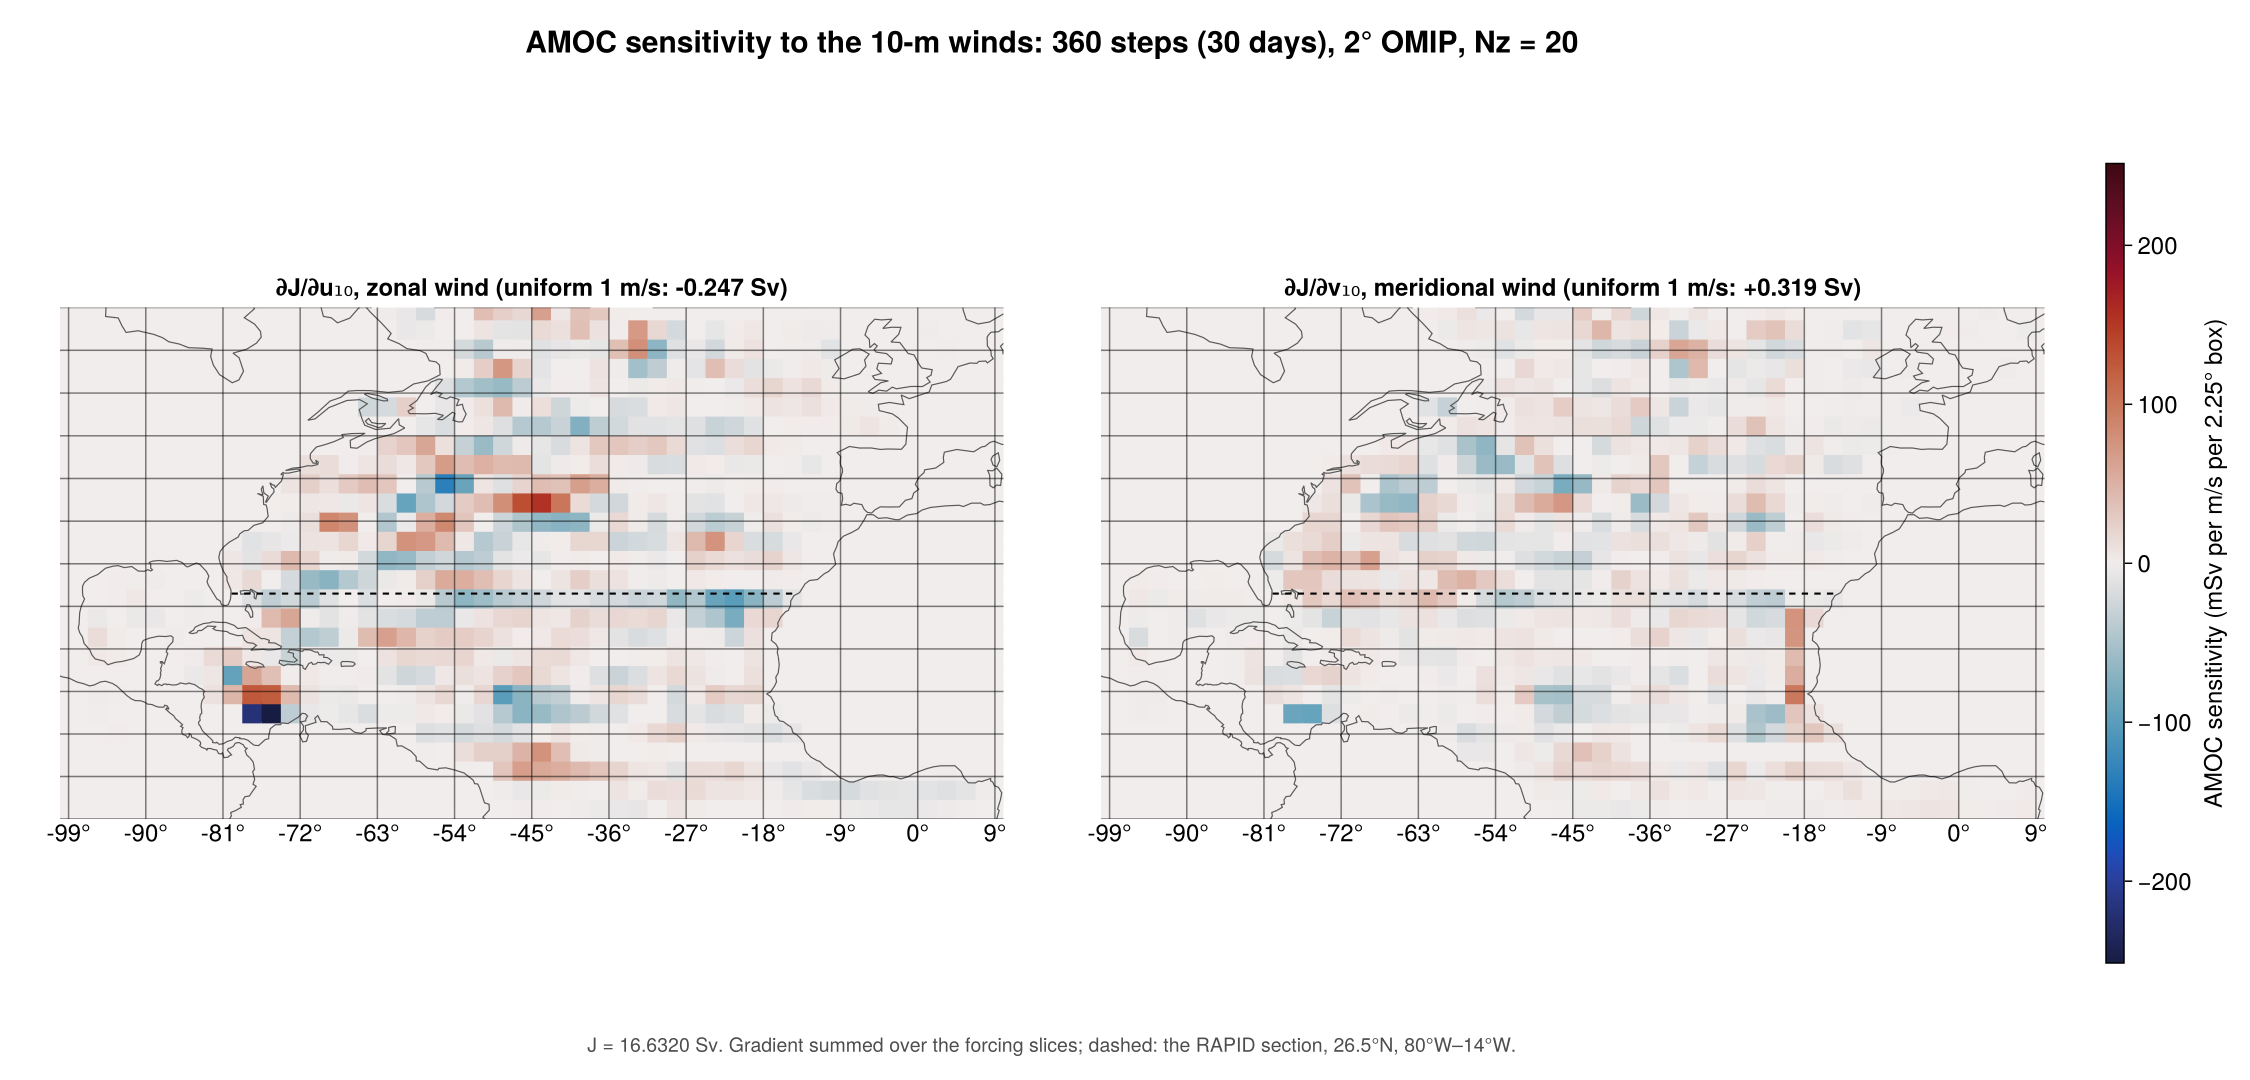
\includegraphics[width=0.84\textwidth,trim=0 60 0 40,clip]{figures/amoc_sensitivity_twodegree_nz20_360step.png}
\caption{Sensitivity of $J$ after 30 days to the zonal (left) and meridional (right) \SI{10}{m} wind, summed over the
window's forcing slices (the response to a wind perturbation held for the whole window), in \ang{2.25} boxes.
Dashed: the RAPID section.}
\label{fig:map}
\end{figure}

After one week the zonal-wind sensitivity lies in zonal bands along and just south of the section, as
expected from Ekman transport. The meridional-wind sensitivity is concentrated at the African coast near
\ang{18}W. By 30 days (Fig.~\ref{fig:map}) the pattern has broken into isolated boxes, the largest in the
Caribbean. The response to a uniform \SI{1}{m/s} zonal wind falls from \SI{-1.58}{Sv} at one week to
\SI{-0.25}{Sv}, while the largest box value grows. The runs start from rest, so these windows sample the
adjustment from rest, not equilibrium sensitivity.

\begin{center}\small
\begin{tabular}{@{}lrr@{}}
\toprule
Frozen against full mixing in the adjoint & 84 steps & 360 steps \\
\midrule
cosine(full, frozen); norm ratio & 0.99964; 0.996 & 0.99418; 0.990 \\
error vs.\ FD secant along $d_{\text{full}}$ ($h = 1/32$--$1$): full / frozen & $-0.6$ / $-1.0\,\%$ & $-0.2$ / $-1.7\,\%$ \\
error vs.\ FD secant along $d_{\text{frozen}}$: full / frozen & $-0.1$ / $-0.4\,\%$ & $-1.0$ / $-1.3\,\%$ \\
uniform \SI{1}{m/s} $v_{10}$ response, full / frozen [Sv] & $+0.05$ / $+0.12$ & $+0.32$ / $+0.76$ \\
compile; first call; repeat call (frozen) & \SI{29}{min}; \SI{2675}{s}; \SI{27}{s} & \SI{30}{min}; \SI{2475}{s}; \SI{114}{s} \\
\bottomrule
\end{tabular}
\end{center}

In all four comparisons the full adjoint is the better predictor of the finite response, and freezing
saves no time. So, unlike ReactOcean, where the exact CATKE gradient grew without bound within ten
days, this model does not need frozen mixing at 30 days. The two gradients are nearly parallel, but
their uniform-wind sums differ by $2.4\times$, because those sums cancel large values of both signs, and
the full gradient's Caribbean peak is absent from the frozen one. A finite-difference test along the uniform-wind directions would settle which is right.

\section*{Cost (one A100, compiled once per configuration)}

\begin{center}\small
\begin{tabular}{@{}lrrrr@{}}
\toprule
& 2 steps & 8 steps & 84 steps & 360 steps \\
\midrule
model build & \SI{916}{s} & \SI{931}{s} & \SI{1022}{s} & \SI{1423}{s} \\
gradient compile & \SI{27.1}{min} & \SI{28.4}{min} & \SI{27.3}{min} & \SI{29.1}{min} \\
first call / repeat call & \SI{2368}{s} / \SI{0.8}{s} & \SI{2350}{s} / \SI{3.5}{s} & \SI{2241}{s} / \SI{28}{s} & \SI{2367}{s} / \SI{104}{s} \\
\bottomrule
\end{tabular}
\end{center}
The first call's \SI{\sim 39}{min} is host-side, most likely Julia compiling the compiled functions' call
wrappers for the large model type (\SI{13}{min} for the smaller ECCO4-forced model).

\section*{In progress and next steps}

\begin{enumerate}
  \item \textbf{Lead-time sensitivity after Pillar et al.\ (2016, Fig.~1)}, with forcing B. Its monthly
        slices give one row per lead: rows of $-1$, $-2$, $-3$ months for 90 days, and $-1$, $-3$, $-6$,
        $-12$ months for a year. Columns are zonal and meridional stress, heat flux (upward positive) and
        freshwater flux (evaporation positive), per unit area. 90-day runs with full and frozen mixing, and a
        1-year run, are queued on Lonestar6. The averaged objective is verified at 8 steps.
  \item Finite differences along uniform-wind directions at 30 days, to settle the full vs.\ frozen sums.
  \item A spun-up initial state and Nz = 70. With forcing A beyond 30 days the in-memory 3-hourly forcing
        and its adjoint copy outgrow one GPU, an estimated \SI{86}{GB} for a year; forcing B avoids this.
\end{enumerate}

\end{document}
